\documentclass[9pt]{beamer}
\mode<presentation>
\usepackage[T1]{fontenc}
\usepackage{color}
\usepackage{graphicx}
\usepackage{natbib}
\usepackage{tikz}
\usetikzlibrary{shapes.geometric}
\usepackage{xmpmulti}
\usepackage{animate}
\usepackage{tcolorbox}
\usepackage{amsmath}
\usepackage{gensymb}
\usepackage{csquotes}
\usepackage{bibentry}
\nobibliography*

\usetheme{Singapore}
%\usecolortheme{seahorse}

\usefonttheme{professionalfonts}

\title[Word \& Doc Embeddings]{A Rapid Computer-assisted Systematic Map of Regional Climate Impacts}
%\author{Max Callaghan, Gerritt }
\institute[MCC]{
	
\includegraphics[height=1cm,width=2cm]{images/MCC_Logo_RZ_rgb.jpg} \hspace{5em} 
\includegraphics[height=1cm]{images/climate_analytics.png}
}

\newif\ifframeinlbf
\frameinlbftrue
\makeatletter
\newcommand\listofframes{\@starttoc{lbf}}
\makeatother

\addtobeamertemplate{frametitle}{}{%
	\ifframeinlbf
	\addcontentsline{lbf}{section}{\protect\makebox[2em][l]{%
			\protect\usebeamercolor[fg]{structure}\insertframenumber\hfill}%
		\insertframetitle\par}%
	\else\fi
}

\newtheorem*{remark}{}

\bibliographystyle{apalike}

\begin{document}
	


\begin{frame}{We predict the relevance of a document most of the time}
\begin{figure}
	\begin{columns}
		\begin{column}{0.3812\linewidth}
			\begin{figure}
					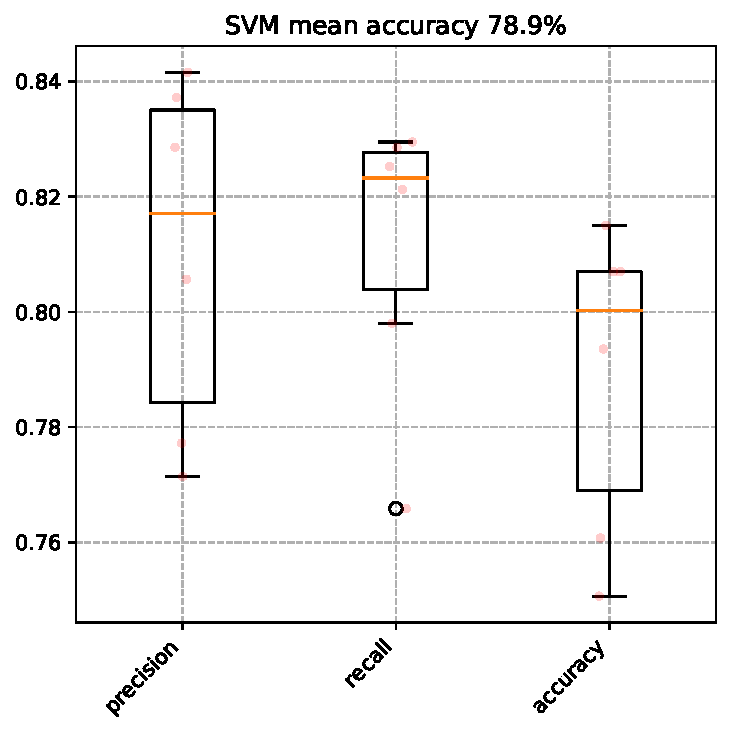
\includegraphics[width=\linewidth]{../plots/prediction_models/relevance_prediction_2020-05-12.pdf}
			\end{figure}
			\begin{figure}
				\only<1>{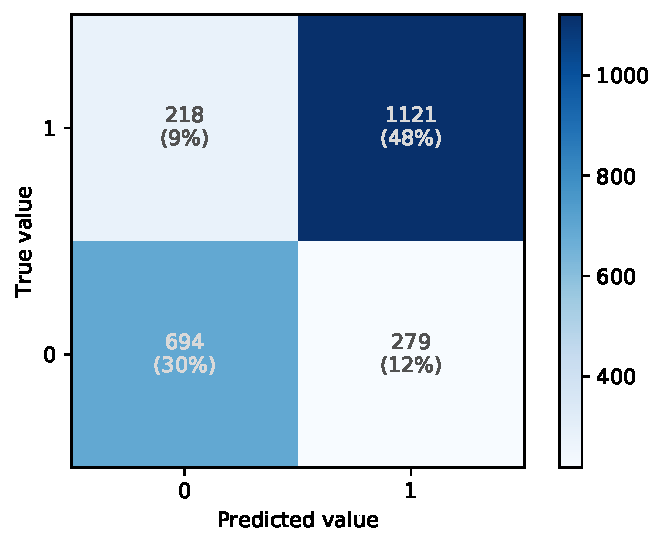
\includegraphics[width=\linewidth]{../plots/prediction_models/relevance_confusion.pdf}}
			\end{figure}
		\end{column}
		\begin{column}{0.5\linewidth}
			Humans were a little more accurate than our model on average, but the distribution was greater.
			\only<1>{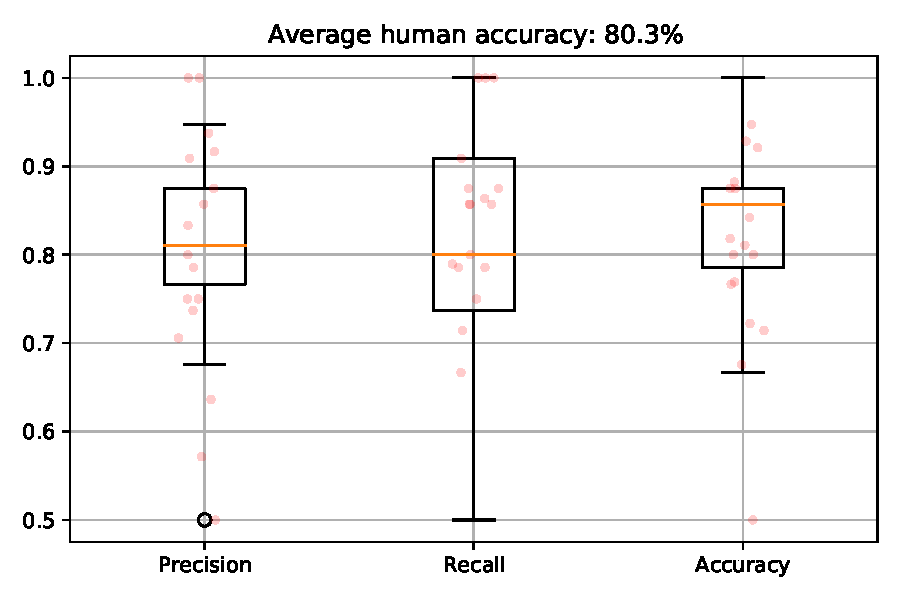
\includegraphics[width=\linewidth]{../plots/human_accuracy.pdf}}
		\end{column}
	\end{columns}

\end{figure}
\end{frame}

\end{document}